\documentclass[twoside]{book}

% Packages required by doxygen
\usepackage{fixltx2e}
\usepackage{calc}
\usepackage{doxygen}
\usepackage[export]{adjustbox} % also loads graphicx
\usepackage{graphicx}
\usepackage[utf8]{inputenc}
\usepackage{makeidx}
\usepackage{multicol}
\usepackage{multirow}
\PassOptionsToPackage{warn}{textcomp}
\usepackage{textcomp}
\usepackage[nointegrals]{wasysym}
\usepackage[table]{xcolor}

% Font selection
\usepackage[T1]{fontenc}
\usepackage[scaled=.90]{helvet}
\usepackage{courier}
\usepackage{amssymb}
\usepackage{sectsty}
\renewcommand{\familydefault}{\sfdefault}
\allsectionsfont{%
  \fontseries{bc}\selectfont%
  \color{darkgray}%
}
\renewcommand{\DoxyLabelFont}{%
  \fontseries{bc}\selectfont%
  \color{darkgray}%
}
\newcommand{\+}{\discretionary{\mbox{\scriptsize$\hookleftarrow$}}{}{}}

% Page & text layout
\usepackage{geometry}
\geometry{%
  a4paper,%
  top=2.5cm,%
  bottom=2.5cm,%
  left=2.5cm,%
  right=2.5cm%
}
\tolerance=750
\hfuzz=15pt
\hbadness=750
\setlength{\emergencystretch}{15pt}
\setlength{\parindent}{0cm}
\setlength{\parskip}{3ex plus 2ex minus 2ex}
\makeatletter
\renewcommand{\paragraph}{%
  \@startsection{paragraph}{4}{0ex}{-1.0ex}{1.0ex}{%
    \normalfont\normalsize\bfseries\SS@parafont%
  }%
}
\renewcommand{\subparagraph}{%
  \@startsection{subparagraph}{5}{0ex}{-1.0ex}{1.0ex}{%
    \normalfont\normalsize\bfseries\SS@subparafont%
  }%
}
\makeatother

% Headers & footers
\usepackage{fancyhdr}
\pagestyle{fancyplain}
\fancyhead[LE]{\fancyplain{}{\bfseries\thepage}}
\fancyhead[CE]{\fancyplain{}{}}
\fancyhead[RE]{\fancyplain{}{\bfseries\leftmark}}
\fancyhead[LO]{\fancyplain{}{\bfseries\rightmark}}
\fancyhead[CO]{\fancyplain{}{}}
\fancyhead[RO]{\fancyplain{}{\bfseries\thepage}}
\fancyfoot[LE]{\fancyplain{}{}}
\fancyfoot[CE]{\fancyplain{}{}}
\fancyfoot[RE]{\fancyplain{}{\bfseries\scriptsize Generated by Doxygen }}
\fancyfoot[LO]{\fancyplain{}{\bfseries\scriptsize Generated by Doxygen }}
\fancyfoot[CO]{\fancyplain{}{}}
\fancyfoot[RO]{\fancyplain{}{}}
\renewcommand{\footrulewidth}{0.4pt}
\renewcommand{\chaptermark}[1]{%
  \markboth{#1}{}%
}
\renewcommand{\sectionmark}[1]{%
  \markright{\thesection\ #1}%
}

% Indices & bibliography
\usepackage{natbib}
\usepackage[titles]{tocloft}
\setcounter{tocdepth}{3}
\setcounter{secnumdepth}{5}
\makeindex

% Hyperlinks (required, but should be loaded last)
\usepackage{ifpdf}
\ifpdf
  \usepackage[pdftex,pagebackref=true]{hyperref}
\else
  \usepackage[ps2pdf,pagebackref=true]{hyperref}
\fi
\hypersetup{%
  colorlinks=true,%
  linkcolor=blue,%
  citecolor=blue,%
  unicode%
}

% Custom commands
\newcommand{\clearemptydoublepage}{%
  \newpage{\pagestyle{empty}\cleardoublepage}%
}

\usepackage{caption}
\captionsetup{labelsep=space,justification=centering,font={bf},singlelinecheck=off,skip=4pt,position=top}

%===== C O N T E N T S =====

\begin{document}

% Titlepage & ToC
\hypersetup{pageanchor=false,
             bookmarksnumbered=true,
             pdfencoding=unicode
            }
\pagenumbering{roman}
\begin{titlepage}
\vspace*{7cm}
\begin{center}%
{\Large My Project }\\
\vspace*{1cm}
{\large Generated by Doxygen 1.8.11}\\
\end{center}
\end{titlepage}
\clearemptydoublepage
\tableofcontents
\clearemptydoublepage
\pagenumbering{arabic}
\hypersetup{pageanchor=true}

%--- Begin generated contents ---
\chapter{Writing documentation for Open\+CV}
\label{tutorial_documentation}
\hypertarget{tutorial_documentation}{}
\#\+The Fast Bilateral Solver ({\bfseries Still in development})

{\bfseries The Bilater Solver} is a novel algorithm for edge-\/aware smoothing that combines the flexibility and speed of simple filtering approaches with the accuracy of domain-\/specific optimization algorithms. This algorithm was presented by Jonathan T. Barron and Ben Poole as an E\+C\+C\+V2016 oral and best paper nominee. Algorithm details and applications can be found in \href{https://arxiv.org/pdf/1511.03296.pdf}{\tt https\+://arxiv.\+org/pdf/1511.\+03296.\+pdf} .







 \subsection*{Introduce}

\subsubsection*{Algorithm}

We begin by presenting the objective and optimization techniques that make up our bilateral solver. Let us assume that we have some per-\/pixel input quantities {\bfseries t} (the “target” value, see Figure 1a) and some per-\/pixel confidence of those quantities {\bfseries c} (Figure 1c), both represented as vectorized images. Let us also assume that we have some “reference” image (Figure 1d), which is a normal R\+GB image. Our goal is to recover an “output” vector x (Figure 1b), which will resemble the input target where the confidence is large while being smooth and tightly aligned to edges in the reference image. We will accomplish this by constructing an optimization problem consisting of an image-\/dependent smoothness term that encourages {\bfseries x} to be bilateral-\/smooth, and a data-\/fidelity term that minimizes the squared residual between x and the target {\bfseries t} weighted by our confidence {\bfseries c}\+: \$\$minimize\{\}\{2\}\{i,j\}\{W\}\+\_\+\{i,j\}(x\+\_\+i-\/x\+\_\+j)$^\wedge$\{2\}+\{i\}(c\+\_\+i-\/t\+\_\+i)$^\wedge$\{2\}  (1)\$\$ The smoothness term in this optimization problem is built around an affinity matrix Ŵ , which is a bistochastized version of a bilateral affinity matrix {\bfseries W} . Each element of the bilateral affinity matrix \$\+W\+\_\+\{i,j\}\$ reflects the affinity between pixels i and j in the reference image in the Y\+UV colorspace\+: \$\$\+W\+\_\+\{i,j\} = (-\/\{ $|$\mbox{[}p\+\_\+i$^\wedge$x,p\+\_\+i$^\wedge$y\mbox{]}-\/\mbox{[}\mbox{[}p\+\_\+j$^\wedge$x,p\+\_\+j$^\wedge$y\mbox{]}\mbox{]} $|$\}\{2\{xy\}$^\wedge$2\}-\/\{(p\+\_\+i$^\wedge$l-\/p\+\_\+j$^\wedge$l)$^\wedge$2\}\{2\{l\}$^\wedge$2\}-\/\{ $|$\mbox{[}p\+\_\+i$^\wedge$u,p\+\_\+i$^\wedge$v\mbox{]}-\/\mbox{[}\mbox{[}p\+\_\+j$^\wedge$u,p\+\_\+j$^\wedge$v\mbox{]}\mbox{]} $|$\}\{2\{uv\}$^\wedge$2\}) (2)\$\$ Where \$p\+\_\+i\$ is a pixel in our reference image with a spatial position \$(p\+\_\+i$^\wedge$x, p\+\_\+i$^\wedge$y )\$ and color \$(p\+\_\+i$^\wedge$l , p\+\_\+i$^\wedge$u , p\+\_\+i$^\wedge$v )\$. The \$\{xy\} , \$ , and \$σ\+\_\+\{uv\}\$ parameters control the extent of the spatial, luma, and chroma support of the filter, respectively. This {\bfseries W} matrix is commonly used in the bilateral filter, an edge-\/preserving filter that blurs within regions but not across edges by locally adapting the filter to the image content. There are techniques for speeding up bilateral filtering which treat the filter as a {\bfseries “splat/blur/slice”} procedure\+: pixel values are “splatted” onto a small set of vertices in a grid or lattice (a soft histogramming operation), then those vertex values are blurred, and then the filtered pixel values are produced via a “slice” (an interpolation) of the blurred vertex values. These splat/blur/slice filtering approaches all correspond to a compact and efficient factorization of {\bfseries W} \+: \$\$W = S$^\wedge$T\{B\}S (3)\$\$ Barron et al. built on this idea to allow for optimization problems to be “splatted” and solved in bilateral-\/space. They use a “simplified” bilateral grid and a technique for producing bistochastization matrices \$\+D\+\_\+n , D\+\_\+m\$ that together give the the following equivalences\+: \$\$\{W\} = S$^\wedge$\+T\+D\+\_\+m$^\wedge$\{-\/1\}D\+\_\+n\{B\}D\+\_\+n\+D\+\_\+m$^\wedge$\{-\/1\}S , S\+S$^\wedge$T = D\+\_\+m (4)\$\$ They also perform a variable substitution, which reformulates a high-\/dimensional pixel-\/space optimization problem in terms of the lower-\/dimensional bilateral-\/space vertices\+: \$\$x = S$^\wedge$\+Ty (5)\$\$ Where y is a small vector of values for each bilateral-\/space vertex, while x is a large vector of values for each pixel. With these tools we can not only reformulate our pixel-\/space loss function in Eq 1 in bilateral-\/space, but we can rewrite that bilateral-\/space loss function in a quadratic form\+: \$\$minimize\{1\}\{2\}y$^\wedge$\+T\+Ay -\/ b$^\wedge$\+Ty + c (6)\$\$ \$\$A = (D\+\_\+m -\/ D\+\_\+n\{B\}D\+\_\+n) + diag(S c)\$\$ \$\$b = S( c   t)\$\$ \$\$c = \{1\}\{2\}( c   t)$^\wedge$T t\$\$ where \$\$ is the Hadamard product. {\bfseries A} derivation of this reformulation can be found in the supplement. While the optimization problem in Equation 1 is intractably expensive to solve naively, in this bilateral-\/space formulation optimization can be performed quickly. Minimizing that quadratic form is equivalent to solving a sparse linear system\+: \$\$\+Ay = b (7)\$\$ We can produce a pixel-\/space solution x̂ by simply slicing the solution to that linear system\+: \$\$\{x\} = S$^\wedge$T(A$^\wedge$\{-\/1\}b)  (8)\$\$ With this we can describe our algorithm, which we will refer to as the “bilateral solver.\+” The input to the solver is a reference R\+GB image, a target image that contains noisy observed quantities which we wish to improve, and a confidence image. We construct a simplified bilateral grid from the reference image, which is bistochastized as in \mbox{[}2\mbox{]} (see the supplement for details), and with that we construct the A matrix and b vector described in Equation 6 which are used to solve the linear system in Equation 8 to produce an output image. If we have multiple target images (with the same reference and confidence images) then we can construct a larger linear system in which b has many columns, and solve for each channel simultaneously using the same A matrix. In this many-\/target case, if b is low rank then that property can be exploited to accelerate optimization, as we show in the supplement.

\subsubsection*{Implementation}


\begin{DoxyItemize}
\item {\bfseries Splat+\+Blur+\+Slice Procedure}  The two bilateral representations we use in this project, here shown filtering a toy one-\/dimensional grayscale image of a step-\/edge. This toy image corresponds to a 2D space visualized here (x = pixel location, y = pixel value) while in the paper we use R\+GB images, which corresponds to a 5D space (X\+Y\+R\+GB). The lattice (Fig 2a) uses barycen-\/tric interpolation to map pixels to vertices and requires d+1 blurring operations, where d is the dimensionality of the space. The simplified bilateral grid (Fig 2b) uses nearest-\/neighbor interpolation and requires d blurring operations which are summed rather than done in sequence. The grid is cheaper to construct and to use than the lattice, but the use of hard assignments means that the filtered output often has blocky piecewise-\/constant artifacts.
\item {\bfseries Diagrammatize} 
\begin{DoxyCode}
1 st=>start: Start
2 e=>end
3 
4 inr=>operation: Imput reference image
5 int=>operation: Imput target image
6 bg=>operation: construct BilateralGrid
7 sl=>operation: construct SliceMatrix
8 bl=>operation: construct BlurMatrix
9 A1=>operation: construct AMatrix step1
10 A2=>operation: construct AMatrix step2
11 cg=>operation: execute ICCG
12 out=>operation: output the resolt
13 
14 
15 st->inr->bg->sl->bl->A1->int->A2->cg->out->e
\end{DoxyCode}

\end{DoxyItemize}

\#\#\#\+Reference 
\begin{DoxyCode}
1 article\{BarronPoole2016,
2 author = \{Jonathan T Barron and Ben Poole\},
3 title = \{The Fast Bilateral Solver\},
4 journal = \{ECCV\},
5 year = \{2016\},
6 \}
7 @article\{Barron2015A,
8 author = \{Jonathan T Barron and Andrew Adams and YiChang Shih and Carlos Hern\(\backslash\)'andez\},
9 title = \{Fast Bilateral-Space Stereo for Synthetic Defocus\},
10 journal = \{CVPR\},
11 year = \{2015\},
12 \}
13 @article\{Adams2010,
14 author = \{Andrew Adams  Jongmin Baek    Abe Davis\},
15 title = \{Fast High-Dimensional Filtering Using the Permutohedral Lattice\},
16 journal = \{Eurographics\},
17 year = \{2010\},
18 \}
\end{DoxyCode}
 

 \subsection*{Installation Instructions}

\subsubsection*{Build Open\+CV}

This is just a suggestion on how to build Open\+CV 3.\+1. There a plenty of options. Also some packages might be optional. 
\begin{DoxyCode}
1 sudo apt-get install libgtk2.0-dev pkg-config libavcodec-dev libavformat-dev libswscale-dev python-dev
       python-numpy libtbb2 libtbb-dev libjpeg-dev libpng-dev libtiff-dev libjasper-dev libdc1394-22-dev
2 git clone https://github.com/Itseez/opencv.git
3 cd opencv
4 mkdir build
5 cd build
6 cmake -D CMAKE\_BUILD\_TYPE=RELEASE -D WITH\_CUDA=OFF ..
7 make -j
8 sudo make install
\end{DoxyCode}


\#\#\#\+Build The\+\_\+\+Bilateral\+\_\+\+Solver 
\begin{DoxyCode}
1 git clone https://github.com/THUKey/The\_Bilateral\_Solver.git
2 cd The\_Bilateral\_Solver/build
3 cmake ..
4 make
\end{DoxyCode}
 This will create three executable demos, that you can run as shown in below.

\paragraph*{Depthsuperresolution}

 the target. 
\begin{DoxyCode}
1 ./Depthsuperres
\end{DoxyCode}
  This result(use bilateral solver) is far from the optimal performance, which means there are some extra work to do, such as to patiently adjustment parameters and to optimize the implementation. 
\begin{DoxyCode}
1 ./Latticefilter reference.png target.png
\end{DoxyCode}
  This result(use permutohedral\+\_\+lattice) is quite nice. \#\#\#\#\+Colorization 
\begin{DoxyCode}
1 ./Colorize rose1.webp
\end{DoxyCode}
  draw image, then press \char`\"{}\+E\+S\+C\char`\"{} twice to launch the colorization procession.  colorized image. you could change the {\bfseries rose1.\+webp} to your own image. Thanks for \href{https://github.com/timuda/colorization_s_demo}{\tt timuda}, his colorization implementation help me a lot.

\#\#\#\#\+Permutohedral\+Lattice\+Filter 
\begin{DoxyCode}
1 ./Latticefilter flower8.jpg
\end{DoxyCode}
 In Barron\textquotesingle{}s another paper {\itshape Fast Bilateral-\/\+Space Stereo for Synthetic Defocus}, both bileteral\+\_\+solver and permutohedral lattice are used to do experiment, and the result shows that bilateral\+\_\+solver is faster than permutohedral lattice technique, but the permutohedral is more accurate than the bilateral\+\_\+solver. In other words, this is the tradeoff between time and accuracy. Actually, both two techniques\textquotesingle{} tradeoff can be worthwhile in appropriate condition. So I want to implement both two technique for more widely use.  filter\+\_\+output.  filter\+\_\+input.



 \subsection*{Basic Usage}

\#\#\# Depthsuperresolution\+: 
\begin{DoxyCode}
1 BilateralGrid BiGr(mat\_R);
2 BiGr.Depthsuperresolution(mat\_R,mat\_T,sigma\_spatial,sigma\_luma,sigma\_chroma);
\end{DoxyCode}
 Firstly, we use the reference image mat\+\_\+R construct a \hyperlink{classBilateralGrid}{Bilateral\+Grid}, the we launch a depthsuperresolution to optimize the target image mat\+\_\+T. The parameter sigma\+\_\+spatial is the Gaussian kernal for coordinate x y, similarly , the sigma\+\_\+luma correspond luma(\+Y) and the sigma\+\_\+chroma correspond chroma(\+U\+V). It need to be noted that he mat\+\_\+R should be covert to Y\+UV form before construct the bilateralgrid.

\#\#\#\+Colorization 
\begin{DoxyCode}
1 InputImage InImg(mat\_in);
2 mat\_bg\_in = InImg.get\_Image(IMG\_YUV);
3 InImg.draw\_Image();
4 mat\_bg\_draw\_in = InImg.get\_Image(IMG\_DRAWYUV);
5 BilateralGrid BiGr(mat\_bg\_in);
6 BiGr.Colorization(mat\_in,mat\_bg\_draw\_in);
\end{DoxyCode}
 Similar to above, we need to covert the imput image mat\+\_\+in(gray image for colorization) to Y\+UV form, then draw the gray image. when the drawing finished, press \char`\"{}\+E\+S\+C\char`\"{} twice to launch the colorization procession. the result will be save in specified folder. \#\#\#\+Permutohedral\+Lattce 
\begin{DoxyCode}
1 bilateral(im,spatialSigma,colorSigma);
\end{DoxyCode}
 Similar to \hyperlink{classBilateralGrid}{Bilateral\+Grid}, the Permutohedral\+Lattce also need spatial parameter and the color parameter to specified the Gaussian kernel.



 \subsection*{Schedule}

\tabulinesep=1mm
\begin{longtabu} spread 0pt [c]{*3{|X[-1]}|}
\hline
\rowcolor{\tableheadbgcolor}{\bf Item }&\PBS\raggedleft {\bf State }&\PBS\centering {\bf Remark  }\\\cline{1-3}
\endfirsthead
\hline
\endfoot
\hline
\rowcolor{\tableheadbgcolor}{\bf Item }&\PBS\raggedleft {\bf State }&\PBS\centering {\bf Remark  }\\\cline{1-3}
\endhead
C++ code of the core algorithm &\PBS\raggedleft Completed &\PBS\centering also python \\\cline{1-3}
Depthsuperres module &\PBS\raggedleft Completed &\PBS\centering need optimize \\\cline{1-3}
Colorization module &\PBS\raggedleft Completed &\PBS\centering choose I\+C\+CG or others \\\cline{1-3}
Permutohedral\+Lattice\+Filter &\PBS\raggedleft Completed &\PBS\centering increse Compatibility \\\cline{1-3}
Semantic Segmentation optimizer &\PBS\raggedleft Ongoing &\PBS\centering try apply in C\+NN \\\cline{1-3}
Contribute project to Open\+CV &\PBS\raggedleft Ongoing &\PBS\centering coding testfile \\\cline{1-3}
Detail Documentation &\PBS\raggedleft Ongoing &\PBS\centering writing toturial \\\cline{1-3}
\end{longtabu}

\chapter{R\+E\+A\+D\+ME}
\label{md_README}
\hypertarget{md_README}{}
\#\+The Fast Bilateral Solver ({\bfseries Still in development})

{\bfseries The Bilater Solver} is a novel algorithm for edge-\/aware smoothing that combines the flexibility and speed of simple filtering approaches with the accuracy of domain-\/specific optimization algorithms. This algorithm was presented by Jonathan T. Barron and Ben Poole as an E\+C\+C\+V2016 oral and best paper nominee. Algorithm details and applications can be found in \href{https://arxiv.org/pdf/1511.03296.pdf}{\tt https\+://arxiv.\+org/pdf/1511.\+03296.\+pdf} .







 \subsection*{Introduce}

\subsubsection*{Algorithm}

We begin by presenting the objective and optimization techniques that make up our bilateral solver. Let us assume that we have some per-\/pixel input quantities {\bfseries t} (the “target” value, see Figure 1a) and some per-\/pixel confidence of those quantities {\bfseries c} (Figure 1c), both represented as vectorized images. Let us also assume that we have some “reference” image (Figure 1d), which is a normal R\+GB image. Our goal is to recover an “output” vector x (Figure 1b), which will resemble the input target where the confidence is large while being smooth and tightly aligned to edges in the reference image. We will accomplish this by constructing an optimization problem consisting of an image-\/dependent smoothness term that encourages {\bfseries x} to be bilateral-\/smooth, and a data-\/fidelity term that minimizes the squared residual between x and the target {\bfseries t} weighted by our confidence {\bfseries c}\+: \$\$minimize\{\}\{2\}\{i,j\}\{W\}\+\_\+\{i,j\}(x\+\_\+i-\/x\+\_\+j)$^\wedge$\{2\}+\{i\}(c\+\_\+i-\/t\+\_\+i)$^\wedge$\{2\}  (1)\$\$ The smoothness term in this optimization problem is built around an affinity matrix Ŵ , which is a bistochastized version of a bilateral affinity matrix {\bfseries W} . Each element of the bilateral affinity matrix \$\+W\+\_\+\{i,j\}\$ reflects the affinity between pixels i and j in the reference image in the Y\+UV colorspace\+: \$\$\+W\+\_\+\{i,j\} = (-\/\{ $|$\mbox{[}p\+\_\+i$^\wedge$x,p\+\_\+i$^\wedge$y\mbox{]}-\/\mbox{[}\mbox{[}p\+\_\+j$^\wedge$x,p\+\_\+j$^\wedge$y\mbox{]}\mbox{]} $|$\}\{2\{xy\}$^\wedge$2\}-\/\{(p\+\_\+i$^\wedge$l-\/p\+\_\+j$^\wedge$l)$^\wedge$2\}\{2\{l\}$^\wedge$2\}-\/\{ $|$\mbox{[}p\+\_\+i$^\wedge$u,p\+\_\+i$^\wedge$v\mbox{]}-\/\mbox{[}\mbox{[}p\+\_\+j$^\wedge$u,p\+\_\+j$^\wedge$v\mbox{]}\mbox{]} $|$\}\{2\{uv\}$^\wedge$2\}) (2)\$\$ Where \$p\+\_\+i\$ is a pixel in our reference image with a spatial position \$(p\+\_\+i$^\wedge$x, p\+\_\+i$^\wedge$y )\$ and color \$(p\+\_\+i$^\wedge$l , p\+\_\+i$^\wedge$u , p\+\_\+i$^\wedge$v )\$. The \$\{xy\} , \$ , and \$σ\+\_\+\{uv\}\$ parameters control the extent of the spatial, luma, and chroma support of the filter, respectively. This {\bfseries W} matrix is commonly used in the bilateral filter, an edge-\/preserving filter that blurs within regions but not across edges by locally adapting the filter to the image content. There are techniques for speeding up bilateral filtering which treat the filter as a {\bfseries “splat/blur/slice”} procedure\+: pixel values are “splatted” onto a small set of vertices in a grid or lattice (a soft histogramming operation), then those vertex values are blurred, and then the filtered pixel values are produced via a “slice” (an interpolation) of the blurred vertex values. These splat/blur/slice filtering approaches all correspond to a compact and efficient factorization of {\bfseries W} \+: \$\$W = S$^\wedge$T\{B\}S (3)\$\$ Barron et al. built on this idea to allow for optimization problems to be “splatted” and solved in bilateral-\/space. They use a “simplified” bilateral grid and a technique for producing bistochastization matrices \$\+D\+\_\+n , D\+\_\+m\$ that together give the the following equivalences\+: \$\$\{W\} = S$^\wedge$\+T\+D\+\_\+m$^\wedge$\{-\/1\}D\+\_\+n\{B\}D\+\_\+n\+D\+\_\+m$^\wedge$\{-\/1\}S , S\+S$^\wedge$T = D\+\_\+m (4)\$\$ They also perform a variable substitution, which reformulates a high-\/dimensional pixel-\/space optimization problem in terms of the lower-\/dimensional bilateral-\/space vertices\+: \$\$x = S$^\wedge$\+Ty (5)\$\$ Where y is a small vector of values for each bilateral-\/space vertex, while x is a large vector of values for each pixel. With these tools we can not only reformulate our pixel-\/space loss function in Eq 1 in bilateral-\/space, but we can rewrite that bilateral-\/space loss function in a quadratic form\+: \$\$minimize\{1\}\{2\}y$^\wedge$\+T\+Ay -\/ b$^\wedge$\+Ty + c (6)\$\$ \$\$A = (D\+\_\+m -\/ D\+\_\+n\{B\}D\+\_\+n) + diag(S c)\$\$ \$\$b = S( c   t)\$\$ \$\$c = \{1\}\{2\}( c   t)$^\wedge$T t\$\$ where \$\$ is the Hadamard product. {\bfseries A} derivation of this reformulation can be found in the supplement. While the optimization problem in Equation 1 is intractably expensive to solve naively, in this bilateral-\/space formulation optimization can be performed quickly. Minimizing that quadratic form is equivalent to solving a sparse linear system\+: \$\$\+Ay = b (7)\$\$ We can produce a pixel-\/space solution x̂ by simply slicing the solution to that linear system\+: \$\$\{x\} = S$^\wedge$T(A$^\wedge$\{-\/1\}b)  (8)\$\$ With this we can describe our algorithm, which we will refer to as the “bilateral solver.\+” The input to the solver is a reference R\+GB image, a target image that contains noisy observed quantities which we wish to improve, and a confidence image. We construct a simplified bilateral grid from the reference image, which is bistochastized as in \mbox{[}2\mbox{]} (see the supplement for details), and with that we construct the A matrix and b vector described in Equation 6 which are used to solve the linear system in Equation 8 to produce an output image. If we have multiple target images (with the same reference and confidence images) then we can construct a larger linear system in which b has many columns, and solve for each channel simultaneously using the same A matrix. In this many-\/target case, if b is low rank then that property can be exploited to accelerate optimization, as we show in the supplement.

\subsubsection*{Implementation}


\begin{DoxyItemize}
\item {\bfseries Splat+\+Blur+\+Slice Procedure}  The two bilateral representations we use in this project, here shown filtering a toy one-\/dimensional grayscale image of a step-\/edge. This toy image corresponds to a 2D space visualized here (x = pixel location, y = pixel value) while in the paper we use R\+GB images, which corresponds to a 5D space (X\+Y\+R\+GB). The lattice (Fig 2a) uses barycen-\/tric interpolation to map pixels to vertices and requires d+1 blurring operations, where d is the dimensionality of the space. The simplified bilateral grid (Fig 2b) uses nearest-\/neighbor interpolation and requires d blurring operations which are summed rather than done in sequence. The grid is cheaper to construct and to use than the lattice, but the use of hard assignments means that the filtered output often has blocky piecewise-\/constant artifacts.
\item {\bfseries Diagrammatize} 
\begin{DoxyCode}
1 st=>start: Start
2 e=>end
3 
4 inr=>operation: Imput reference image
5 int=>operation: Imput target image
6 bg=>operation: construct BilateralGrid
7 sl=>operation: construct SliceMatrix
8 bl=>operation: construct BlurMatrix
9 A1=>operation: construct AMatrix step1
10 A2=>operation: construct AMatrix step2
11 cg=>operation: execute ICCG
12 out=>operation: output the resolt
13 
14 
15 st->inr->bg->sl->bl->A1->int->A2->cg->out->e
\end{DoxyCode}

\end{DoxyItemize}

\#\#\#\+Reference 
\begin{DoxyCode}
1 article\{BarronPoole2016,
2 author = \{Jonathan T Barron and Ben Poole\},
3 title = \{The Fast Bilateral Solver\},
4 journal = \{ECCV\},
5 year = \{2016\},
6 \}
7 @article\{Barron2015A,
8 author = \{Jonathan T Barron and Andrew Adams and YiChang Shih and Carlos Hern\(\backslash\)'andez\},
9 title = \{Fast Bilateral-Space Stereo for Synthetic Defocus\},
10 journal = \{CVPR\},
11 year = \{2015\},
12 \}
13 @article\{Adams2010,
14 author = \{Andrew Adams  Jongmin Baek    Abe Davis\},
15 title = \{Fast High-Dimensional Filtering Using the Permutohedral Lattice\},
16 journal = \{Eurographics\},
17 year = \{2010\},
18 \}
\end{DoxyCode}
 

 \subsection*{Installation Instructions}

\subsubsection*{Build Open\+CV}

This is just a suggestion on how to build Open\+CV 3.\+1. There a plenty of options. Also some packages might be optional. 
\begin{DoxyCode}
1 sudo apt-get install libgtk2.0-dev pkg-config libavcodec-dev libavformat-dev libswscale-dev python-dev
       python-numpy libtbb2 libtbb-dev libjpeg-dev libpng-dev libtiff-dev libjasper-dev libdc1394-22-dev
2 git clone https://github.com/Itseez/opencv.git
3 cd opencv
4 mkdir build
5 cd build
6 cmake -D CMAKE\_BUILD\_TYPE=RELEASE -D WITH\_CUDA=OFF ..
7 make -j
8 sudo make install
\end{DoxyCode}


\#\#\#\+Build The\+\_\+\+Bilateral\+\_\+\+Solver 
\begin{DoxyCode}
1 git clone https://github.com/THUKey/The\_Bilateral\_Solver.git
2 cd The\_Bilateral\_Solver/build
3 cmake ..
4 make
\end{DoxyCode}
 This will create three executable demos, that you can run as shown in below.

\paragraph*{Depthsuperresolution}

 the target. 
\begin{DoxyCode}
1 ./Depthsuperres
\end{DoxyCode}
  This result(use bilateral solver) is far from the optimal performance, which means there are some extra work to do, such as to patiently adjustment parameters and to optimize the implementation. 
\begin{DoxyCode}
1 ./Latticefilter reference.png target.png
\end{DoxyCode}
  This result(use permutohedral\+\_\+lattice) is quite nice. \#\#\#\#\+Colorization 
\begin{DoxyCode}
1 ./Colorize rose1.webp
\end{DoxyCode}
  draw image, then press \char`\"{}\+E\+S\+C\char`\"{} twice to launch the colorization procession.  colorized image. you could change the {\bfseries rose1.\+webp} to your own image. Thanks for \href{https://github.com/timuda/colorization_s_demo}{\tt timuda}, his colorization implementation help me a lot.

\#\#\#\#\+Permutohedral\+Lattice\+Filter 
\begin{DoxyCode}
1 ./Latticefilter flower8.jpg
\end{DoxyCode}
 In Barron\textquotesingle{}s another paper {\itshape Fast Bilateral-\/\+Space Stereo for Synthetic Defocus}, both bileteral\+\_\+solver and permutohedral lattice are used to do experiment, and the result shows that bilateral\+\_\+solver is faster than permutohedral lattice technique, but the permutohedral is more accurate than the bilateral\+\_\+solver. In other words, this is the tradeoff between time and accuracy. Actually, both two techniques\textquotesingle{} tradeoff can be worthwhile in appropriate condition. So I want to implement both two technique for more widely use.  filter\+\_\+output.  filter\+\_\+input.



 \subsection*{Basic Usage}

\#\#\# Depthsuperresolution\+: 
\begin{DoxyCode}
1 BilateralGrid BiGr(mat\_R);
2 BiGr.Depthsuperresolution(mat\_R,mat\_T,sigma\_spatial,sigma\_luma,sigma\_chroma);
\end{DoxyCode}
 Firstly, we use the reference image mat\+\_\+R construct a \hyperlink{classBilateralGrid}{Bilateral\+Grid}, the we launch a depthsuperresolution to optimize the target image mat\+\_\+T. The parameter sigma\+\_\+spatial is the Gaussian kernal for coordinate x y, similarly , the sigma\+\_\+luma correspond luma(\+Y) and the sigma\+\_\+chroma correspond chroma(\+U\+V). It need to be noted that he mat\+\_\+R should be covert to Y\+UV form before construct the bilateralgrid.

\#\#\#\+Colorization 
\begin{DoxyCode}
1 InputImage InImg(mat\_in);
2 mat\_bg\_in = InImg.get\_Image(IMG\_YUV);
3 InImg.draw\_Image();
4 mat\_bg\_draw\_in = InImg.get\_Image(IMG\_DRAWYUV);
5 BilateralGrid BiGr(mat\_bg\_in);
6 BiGr.Colorization(mat\_in,mat\_bg\_draw\_in);
\end{DoxyCode}
 Similar to above, we need to covert the imput image mat\+\_\+in(gray image for colorization) to Y\+UV form, then draw the gray image. when the drawing finished, press \char`\"{}\+E\+S\+C\char`\"{} twice to launch the colorization procession. the result will be save in specified folder. \#\#\#\+Permutohedral\+Lattce 
\begin{DoxyCode}
1 bilateral(im,spatialSigma,colorSigma);
\end{DoxyCode}
 Similar to \hyperlink{classBilateralGrid}{Bilateral\+Grid}, the Permutohedral\+Lattce also need spatial parameter and the color parameter to specified the Gaussian kernel.



 \subsection*{Schedule}

\tabulinesep=1mm
\begin{longtabu} spread 0pt [c]{*3{|X[-1]}|}
\hline
\rowcolor{\tableheadbgcolor}{\bf Item }&\PBS\raggedleft {\bf State }&\PBS\centering {\bf Remark  }\\\cline{1-3}
\endfirsthead
\hline
\endfoot
\hline
\rowcolor{\tableheadbgcolor}{\bf Item }&\PBS\raggedleft {\bf State }&\PBS\centering {\bf Remark  }\\\cline{1-3}
\endhead
C++ code of the core algorithm &\PBS\raggedleft Completed &\PBS\centering also python \\\cline{1-3}
Depthsuperres module &\PBS\raggedleft Completed &\PBS\centering need optimize \\\cline{1-3}
Colorization module &\PBS\raggedleft Completed &\PBS\centering choose I\+C\+CG or others \\\cline{1-3}
Permutohedral\+Lattice\+Filter &\PBS\raggedleft Completed &\PBS\centering increse Compatibility \\\cline{1-3}
Semantic Segmentation optimizer &\PBS\raggedleft Ongoing &\PBS\centering try apply in C\+NN \\\cline{1-3}
Contribute project to Open\+CV &\PBS\raggedleft Ongoing &\PBS\centering coding testfile \\\cline{1-3}
Detail Documentation &\PBS\raggedleft Ongoing &\PBS\centering writing toturial \\\cline{1-3}
\end{longtabu}

\chapter{Hierarchical Index}
\section{Class Hierarchy}
This inheritance list is sorted roughly, but not completely, alphabetically\+:\begin{DoxyCompactList}
\item Algorithm\begin{DoxyCompactList}
\item \contentsline{section}{cv\+:\+:xim\+:\+:Fast\+Bilateral\+Solver\+Filter}{\pageref{classcv_1_1xim_1_1FastBilateralSolverFilter}}{}
\begin{DoxyCompactList}
\item \contentsline{section}{cv\+:\+:xim\+:\+:Fast\+Bilateral\+Solver\+Filter\+Impl}{\pageref{classcv_1_1xim_1_1FastBilateralSolverFilterImpl}}{}
\end{DoxyCompactList}
\end{DoxyCompactList}
\item \contentsline{section}{Bilateral\+Grid}{\pageref{classBilateralGrid}}{}
\item \contentsline{section}{Hash\+Table\+Permutohedral}{\pageref{classHashTablePermutohedral}}{}
\item \contentsline{section}{Input\+Image}{\pageref{classInputImage}}{}
\item \contentsline{section}{Permutohedral\+Lattice}{\pageref{classPermutohedralLattice}}{}
\item \contentsline{section}{st\+\_\+A}{\pageref{structst__A}}{}
\item \contentsline{section}{st\+\_\+blur}{\pageref{structst__blur}}{}
\item \contentsline{section}{st\+\_\+calc}{\pageref{structst__calc}}{}
\item \contentsline{section}{st\+\_\+index}{\pageref{structst__index}}{}
\item \contentsline{section}{st\+\_\+splat}{\pageref{structst__splat}}{}
\item \contentsline{section}{st\+\_\+table}{\pageref{structst__table}}{}
\item \contentsline{section}{str\+\_\+\+C\+SR}{\pageref{structstr__CSR}}{}
\item \contentsline{section}{str\+\_\+\+C\+S\+R\+\_\+colsort}{\pageref{structstr__CSR__colsort}}{}
\end{DoxyCompactList}

\chapter{Class Index}
\section{Class List}
Here are the classes, structs, unions and interfaces with brief descriptions\+:\begin{DoxyCompactList}
\item\contentsline{section}{\hyperlink{classBilateralGrid}{Bilateral\+Grid} }{\pageref{classBilateralGrid}}{}
\item\contentsline{section}{\hyperlink{classcv_1_1xim_1_1FastBilateralSolverFilter}{cv\+::xim\+::\+Fast\+Bilateral\+Solver\+Filter} }{\pageref{classcv_1_1xim_1_1FastBilateralSolverFilter}}{}
\item\contentsline{section}{\hyperlink{classcv_1_1xim_1_1FastBilateralSolverFilterImpl}{cv\+::xim\+::\+Fast\+Bilateral\+Solver\+Filter\+Impl} }{\pageref{classcv_1_1xim_1_1FastBilateralSolverFilterImpl}}{}
\item\contentsline{section}{\hyperlink{classHashTablePermutohedral}{Hash\+Table\+Permutohedral} }{\pageref{classHashTablePermutohedral}}{}
\item\contentsline{section}{\hyperlink{classInputImage}{Input\+Image} }{\pageref{classInputImage}}{}
\item\contentsline{section}{\hyperlink{classPermutohedralLattice}{Permutohedral\+Lattice} }{\pageref{classPermutohedralLattice}}{}
\item\contentsline{section}{\hyperlink{structst__A}{st\+\_\+A} }{\pageref{structst__A}}{}
\item\contentsline{section}{\hyperlink{structst__blur}{st\+\_\+blur} }{\pageref{structst__blur}}{}
\item\contentsline{section}{\hyperlink{structst__calc}{st\+\_\+calc} }{\pageref{structst__calc}}{}
\item\contentsline{section}{\hyperlink{structst__index}{st\+\_\+index} }{\pageref{structst__index}}{}
\item\contentsline{section}{\hyperlink{structst__splat}{st\+\_\+splat} }{\pageref{structst__splat}}{}
\item\contentsline{section}{\hyperlink{structst__table}{st\+\_\+table} }{\pageref{structst__table}}{}
\item\contentsline{section}{\hyperlink{structstr__CSR}{str\+\_\+\+C\+SR} }{\pageref{structstr__CSR}}{}
\item\contentsline{section}{\hyperlink{structstr__CSR__colsort}{str\+\_\+\+C\+S\+R\+\_\+colsort} }{\pageref{structstr__CSR__colsort}}{}
\end{DoxyCompactList}

\chapter{Class Documentation}
\hypertarget{classBilateralGrid}{}\section{Bilateral\+Grid Class Reference}
\label{classBilateralGrid}\index{Bilateral\+Grid@{Bilateral\+Grid}}
\subsection*{Public Member Functions}
\begin{DoxyCompactItemize}
\item 
{\bfseries Bilateral\+Grid} (Mat3f mat\+\_\+image)\hypertarget{classBilateralGrid_a1e1c37f803f6f1fbf9ce75cb999e72e2}{}\label{classBilateralGrid_a1e1c37f803f6f1fbf9ce75cb999e72e2}

\item 
void {\bfseries Depthsuperresolution} (Mat3f mat\+\_\+R, Mat1f mat\+\_\+T, int sigma\+\_\+spatial, int sigma\+\_\+luma, int sigma\+\_\+chroma)\hypertarget{classBilateralGrid_a4cb7eb9613559c1ff6dd38b4b18b39b5}{}\label{classBilateralGrid_a4cb7eb9613559c1ff6dd38b4b18b39b5}

\item 
void {\bfseries Colorization} (Mat3f mat\+\_\+in, Mat3f mat\+\_\+bg\+\_\+draw\+\_\+in)\hypertarget{classBilateralGrid_ad902695cabed0ecafe4237f84a1989b4}{}\label{classBilateralGrid_ad902695cabed0ecafe4237f84a1989b4}

\item 
void {\bfseries Permutohedral\+Lattice} (Mat3f mat\+\_\+in)\hypertarget{classBilateralGrid_a93079277bd1c2e12cbc4d087f3222c7b}{}\label{classBilateralGrid_a93079277bd1c2e12cbc4d087f3222c7b}

\item 
void {\bfseries set\+\_\+\+Draw\+Image} (Mat3f mat\+\_\+draw\+\_\+image)\hypertarget{classBilateralGrid_ac04cb21d31b6698f6aa60ae6cc2bbe34}{}\label{classBilateralGrid_ac04cb21d31b6698f6aa60ae6cc2bbe34}

\item 
void {\bfseries set\+\_\+\+Depth\+Image} (Mat1f mat\+\_\+depth\+\_\+image)\hypertarget{classBilateralGrid_a7ad1f4ecc735e43bbfcc337336ab10bf}{}\label{classBilateralGrid_a7ad1f4ecc735e43bbfcc337336ab10bf}

\item 
void {\bfseries construct\+\_\+\+Slice\+Matrix} (void)\hypertarget{classBilateralGrid_a3133f8c767f4065da5832d54bb7d9278}{}\label{classBilateralGrid_a3133f8c767f4065da5832d54bb7d9278}

\item 
void {\bfseries construct\+\_\+\+Slice\+Matrix\+\_\+for\+\_\+depth} (void)\hypertarget{classBilateralGrid_a4580d6b5b09695abeed154e444199da6}{}\label{classBilateralGrid_a4580d6b5b09695abeed154e444199da6}

\item 
void {\bfseries construct\+\_\+\+Blur\+Matrix} (void)\hypertarget{classBilateralGrid_acfed5846fa5f065305cfeede437c6821}{}\label{classBilateralGrid_acfed5846fa5f065305cfeede437c6821}

\item 
void {\bfseries construct\+\_\+\+A\+Matrix\+\_\+step1} (void)\hypertarget{classBilateralGrid_aabcfb752e903cb30efa74777e9909ff1}{}\label{classBilateralGrid_aabcfb752e903cb30efa74777e9909ff1}

\item 
void {\bfseries construct\+\_\+\+A\+Matrix\+\_\+step2} (void)\hypertarget{classBilateralGrid_a4f07fcdfa8cbe46c7b11fd00a124d7ef}{}\label{classBilateralGrid_a4f07fcdfa8cbe46c7b11fd00a124d7ef}

\item 
void {\bfseries construct\+\_\+\+A\+Matrix\+\_\+step2\+\_\+for\+\_\+depth} ()\hypertarget{classBilateralGrid_aae40be0d1c4edb17db1079bb1612128a}{}\label{classBilateralGrid_aae40be0d1c4edb17db1079bb1612128a}

\item 
void {\bfseries show\+\_\+\+Image} (int num)\hypertarget{classBilateralGrid_a04c894dbca4da5b7a5092b33f9c79b92}{}\label{classBilateralGrid_a04c894dbca4da5b7a5092b33f9c79b92}

\item 
void {\bfseries execute\+\_\+\+Filter} (void)\hypertarget{classBilateralGrid_a2fa58bb40362b25f47073aba74a5ef2f}{}\label{classBilateralGrid_a2fa58bb40362b25f47073aba74a5ef2f}

\item 
void {\bfseries calc\+\_\+\+Bistochastic} (void)\hypertarget{classBilateralGrid_ab873f086735b472feef706f6d9148d46}{}\label{classBilateralGrid_ab873f086735b472feef706f6d9148d46}

\item 
void {\bfseries execute\+\_\+\+Bistochastic} (void)\hypertarget{classBilateralGrid_aff60989adce9c1997a2dc070c0aafce5}{}\label{classBilateralGrid_aff60989adce9c1997a2dc070c0aafce5}

\item 
void {\bfseries execute\+\_\+\+I\+C\+CG} (int iter, float eps)\hypertarget{classBilateralGrid_a701074fe8ec52700a9dfc5dabe030b91}{}\label{classBilateralGrid_a701074fe8ec52700a9dfc5dabe030b91}

\item 
void {\bfseries execute\+\_\+\+I\+C\+C\+G\+\_\+for\+\_\+depth} (int iter, float eps)\hypertarget{classBilateralGrid_a3fe3e289809b9b6709928003e8d58c5e}{}\label{classBilateralGrid_a3fe3e289809b9b6709928003e8d58c5e}

\item 
Mat3f {\bfseries get\+\_\+\+Image} (int num)\hypertarget{classBilateralGrid_a2e69ac4ee7c55b75f5128e78fa8bc319}{}\label{classBilateralGrid_a2e69ac4ee7c55b75f5128e78fa8bc319}

\end{DoxyCompactItemize}


The documentation for this class was generated from the following files\+:\begin{DoxyCompactItemize}
\item 
Bilateral\+Grid.\+hpp\item 
Bilateral\+Grid.\+cpp\end{DoxyCompactItemize}

\hypertarget{classcv_1_1xim_1_1FastBilateralSolverFilter}{}\section{cv\+:\+:xim\+:\+:Fast\+Bilateral\+Solver\+Filter Class Reference}
\label{classcv_1_1xim_1_1FastBilateralSolverFilter}\index{cv\+::xim\+::\+Fast\+Bilateral\+Solver\+Filter@{cv\+::xim\+::\+Fast\+Bilateral\+Solver\+Filter}}


Inheritance diagram for cv\+:\+:xim\+:\+:Fast\+Bilateral\+Solver\+Filter\+:
\nopagebreak
\begin{figure}[H]
\begin{center}
\leavevmode
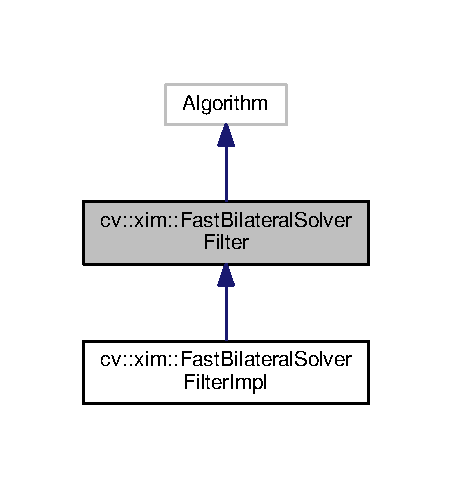
\includegraphics[width=217pt]{classcv_1_1xim_1_1FastBilateralSolverFilter__inherit__graph}
\end{center}
\end{figure}


Collaboration diagram for cv\+:\+:xim\+:\+:Fast\+Bilateral\+Solver\+Filter\+:
\nopagebreak
\begin{figure}[H]
\begin{center}
\leavevmode
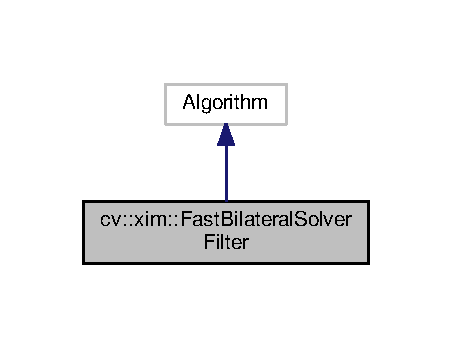
\includegraphics[width=217pt]{classcv_1_1xim_1_1FastBilateralSolverFilter__coll__graph}
\end{center}
\end{figure}
\subsection*{Public Member Functions}
\begin{DoxyCompactItemize}
\item 
virtual C\+V\+\_\+\+W\+R\+AP void {\bfseries filter} (Input\+Array src, Input\+Array confidence, Output\+Array dst)=0\hypertarget{classcv_1_1xim_1_1FastBilateralSolverFilter_ad5361179e54020630af33c08b713a0d2}{}\label{classcv_1_1xim_1_1FastBilateralSolverFilter_ad5361179e54020630af33c08b713a0d2}

\end{DoxyCompactItemize}


The documentation for this class was generated from the following file\+:\begin{DoxyCompactItemize}
\item 
Bilateral\+Solver.\+hpp\end{DoxyCompactItemize}

\hypertarget{classcv_1_1xim_1_1FastBilateralSolverFilterImpl}{}\section{cv\+:\+:xim\+:\+:Fast\+Bilateral\+Solver\+Filter\+Impl Class Reference}
\label{classcv_1_1xim_1_1FastBilateralSolverFilterImpl}\index{cv\+::xim\+::\+Fast\+Bilateral\+Solver\+Filter\+Impl@{cv\+::xim\+::\+Fast\+Bilateral\+Solver\+Filter\+Impl}}


Inheritance diagram for cv\+:\+:xim\+:\+:Fast\+Bilateral\+Solver\+Filter\+Impl\+:
\nopagebreak
\begin{figure}[H]
\begin{center}
\leavevmode
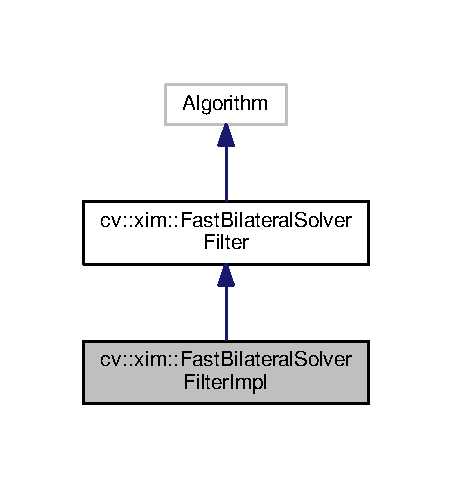
\includegraphics[width=217pt]{classcv_1_1xim_1_1FastBilateralSolverFilterImpl__inherit__graph}
\end{center}
\end{figure}


Collaboration diagram for cv\+:\+:xim\+:\+:Fast\+Bilateral\+Solver\+Filter\+Impl\+:
\nopagebreak
\begin{figure}[H]
\begin{center}
\leavevmode
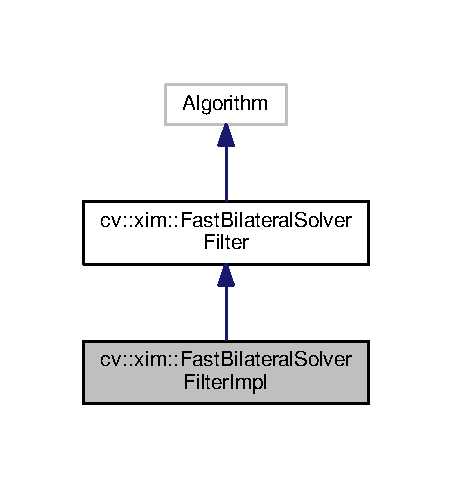
\includegraphics[width=217pt]{classcv_1_1xim_1_1FastBilateralSolverFilterImpl__coll__graph}
\end{center}
\end{figure}
\subsection*{Public Member Functions}
\begin{DoxyCompactItemize}
\item 
void {\bfseries filter} (Input\+Array \&src, Input\+Array \&confidence, Output\+Array \&dst)\hypertarget{classcv_1_1xim_1_1FastBilateralSolverFilterImpl_a660539579f1037e0725732afca096aa6}{}\label{classcv_1_1xim_1_1FastBilateralSolverFilterImpl_a660539579f1037e0725732afca096aa6}

\item 
void {\bfseries solve} (cv\+::\+Mat \&src, cv\+::\+Mat \&confidence, cv\+::\+Mat \&dst)\hypertarget{classcv_1_1xim_1_1FastBilateralSolverFilterImpl_a27d02f3df6c11dd6304ef054ff63ab97}{}\label{classcv_1_1xim_1_1FastBilateralSolverFilterImpl_a27d02f3df6c11dd6304ef054ff63ab97}

\item 
void {\bfseries init} (cv\+::\+Mat \&reference\+\_\+bgr, double sigma\+\_\+spatial, double sigma\+\_\+luma, double sigma\+\_\+chroma)\hypertarget{classcv_1_1xim_1_1FastBilateralSolverFilterImpl_a3ab6f356d5d0144603df413f50c1a065}{}\label{classcv_1_1xim_1_1FastBilateralSolverFilterImpl_a3ab6f356d5d0144603df413f50c1a065}

\item 
void {\bfseries Splat} (Eigen\+::\+Vector\+Xf \&input, Eigen\+::\+Vector\+Xf \&dst)\hypertarget{classcv_1_1xim_1_1FastBilateralSolverFilterImpl_ac59559b02ff6c5a38aa6267ac4022b4b}{}\label{classcv_1_1xim_1_1FastBilateralSolverFilterImpl_ac59559b02ff6c5a38aa6267ac4022b4b}

\item 
void {\bfseries Blur} (Eigen\+::\+Vector\+Xf \&input, Eigen\+::\+Vector\+Xf \&dst)\hypertarget{classcv_1_1xim_1_1FastBilateralSolverFilterImpl_a19104a1f829466a4f8fdacbb508e2029}{}\label{classcv_1_1xim_1_1FastBilateralSolverFilterImpl_a19104a1f829466a4f8fdacbb508e2029}

\item 
void {\bfseries Slice} (Eigen\+::\+Vector\+Xf \&input, Eigen\+::\+Vector\+Xf \&dst)\hypertarget{classcv_1_1xim_1_1FastBilateralSolverFilterImpl_ab7f469c0e32d5c694d3f9ed75c2896b0}{}\label{classcv_1_1xim_1_1FastBilateralSolverFilterImpl_ab7f469c0e32d5c694d3f9ed75c2896b0}

\end{DoxyCompactItemize}
\subsection*{Static Public Member Functions}
\begin{DoxyCompactItemize}
\item 
static Ptr$<$ \hyperlink{classcv_1_1xim_1_1FastBilateralSolverFilterImpl}{Fast\+Bilateral\+Solver\+Filter\+Impl} $>$ {\bfseries create} (Input\+Array guide, double sigma\+\_\+spatial, double sigma\+\_\+luma, double sigma\+\_\+chroma)\hypertarget{classcv_1_1xim_1_1FastBilateralSolverFilterImpl_af921ce7f4381f8c1882ba9b6ebfe46e5}{}\label{classcv_1_1xim_1_1FastBilateralSolverFilterImpl_af921ce7f4381f8c1882ba9b6ebfe46e5}

\end{DoxyCompactItemize}


The documentation for this class was generated from the following file\+:\begin{DoxyCompactItemize}
\item 
Bilateral\+Solver.\+hpp\end{DoxyCompactItemize}

\hypertarget{classHashTablePermutohedral}{}\section{Hash\+Table\+Permutohedral Class Reference}
\label{classHashTablePermutohedral}\index{Hash\+Table\+Permutohedral@{Hash\+Table\+Permutohedral}}
\subsection*{Public Member Functions}
\begin{DoxyCompactItemize}
\item 
{\bfseries Hash\+Table\+Permutohedral} (int kd, int vd)\hypertarget{classHashTablePermutohedral_aacba6988ff20b3238661b551c4e2f0db}{}\label{classHashTablePermutohedral_aacba6988ff20b3238661b551c4e2f0db}

\item 
int {\bfseries size} ()\hypertarget{classHashTablePermutohedral_a9e0fe5faead11889fde71fe9d4f31ef3}{}\label{classHashTablePermutohedral_a9e0fe5faead11889fde71fe9d4f31ef3}

\item 
vector$<$ short $>$ \& {\bfseries get\+Keys} ()\hypertarget{classHashTablePermutohedral_ab2c34c1a7ee93f7f90f7990947de19b2}{}\label{classHashTablePermutohedral_ab2c34c1a7ee93f7f90f7990947de19b2}

\item 
vector$<$ float $>$ \& {\bfseries get\+Values} ()\hypertarget{classHashTablePermutohedral_a0ae627d11ee3f81de2a9ec5c6a08bf57}{}\label{classHashTablePermutohedral_a0ae627d11ee3f81de2a9ec5c6a08bf57}

\item 
float $\ast$ {\bfseries lookup} (const vector$<$ short $>$ \&key, bool create=true)\hypertarget{classHashTablePermutohedral_a48b76ae6d8f0d5140731d3ba1ccee2c4}{}\label{classHashTablePermutohedral_a48b76ae6d8f0d5140731d3ba1ccee2c4}

\item 
size\+\_\+t {\bfseries hash} (const short $\ast$key)\hypertarget{classHashTablePermutohedral_a009a7e5293898ee2f2d823f1d0509dbf}{}\label{classHashTablePermutohedral_a009a7e5293898ee2f2d823f1d0509dbf}

\end{DoxyCompactItemize}


The documentation for this class was generated from the following file\+:\begin{DoxyCompactItemize}
\item 
permutohedral\+\_\+lattice.\+cpp\end{DoxyCompactItemize}

\hypertarget{classInputImage}{}\section{Input\+Image Class Reference}
\label{classInputImage}\index{Input\+Image@{Input\+Image}}
\subsection*{Public Member Functions}
\begin{DoxyCompactItemize}
\item 
{\bfseries Input\+Image} (Mat1f mat\+\_\+image)\hypertarget{classInputImage_a37454b8778c2dfc528a5cd7e25916181}{}\label{classInputImage_a37454b8778c2dfc528a5cd7e25916181}

\item 
{\bfseries Input\+Image} (Mat3f mat\+\_\+image)\hypertarget{classInputImage_a5a6e1d33c07d55cd3412146e83d4db9e}{}\label{classInputImage_a5a6e1d33c07d55cd3412146e83d4db9e}

\item 
{\bfseries Input\+Image} (Mat3f mat\+\_\+image, Mat3f mat\+\_\+image\+\_\+reference)\hypertarget{classInputImage_af9b40c22378994b2ef4005434c4c2a18}{}\label{classInputImage_af9b40c22378994b2ef4005434c4c2a18}

\item 
Mat3f {\bfseries get\+\_\+\+Image} (int num)\hypertarget{classInputImage_a108d36633c6e3aa5e3742d4083984245}{}\label{classInputImage_a108d36633c6e3aa5e3742d4083984245}

\item 
void {\bfseries draw\+\_\+\+Image} (void)\hypertarget{classInputImage_ae9ee4181b5e0dcee6dea4ed1fd0c96f9}{}\label{classInputImage_ae9ee4181b5e0dcee6dea4ed1fd0c96f9}

\item 
void {\bfseries show\+\_\+\+Image} (int num)\hypertarget{classInputImage_afd2a54bf7bdd3f0a964d2e20d320951f}{}\label{classInputImage_afd2a54bf7bdd3f0a964d2e20d320951f}

\end{DoxyCompactItemize}


The documentation for this class was generated from the following files\+:\begin{DoxyCompactItemize}
\item 
Input\+Image.\+hpp\item 
Input\+Image.\+cpp\end{DoxyCompactItemize}

\hypertarget{classPermutohedralLattice}{}\section{Permutohedral\+Lattice Class Reference}
\label{classPermutohedralLattice}\index{Permutohedral\+Lattice@{Permutohedral\+Lattice}}
\subsection*{Public Member Functions}
\begin{DoxyCompactItemize}
\item 
{\bfseries Permutohedral\+Lattice} (int pd, int vd, int n)\hypertarget{classPermutohedralLattice_a4d5de5acf49dd95a3e418fd3a8e90bbe}{}\label{classPermutohedralLattice_a4d5de5acf49dd95a3e418fd3a8e90bbe}

\item 
void {\bfseries splat} (const float $\ast$position, const float $\ast$value)\hypertarget{classPermutohedralLattice_a58fa5f5023232923df3753797c1b89f1}{}\label{classPermutohedralLattice_a58fa5f5023232923df3753797c1b89f1}

\item 
void {\bfseries begin\+Slice} ()\hypertarget{classPermutohedralLattice_a68eba6292f3982c46897bae3f7d2b474}{}\label{classPermutohedralLattice_a68eba6292f3982c46897bae3f7d2b474}

\item 
void {\bfseries slice} (float $\ast$col)\hypertarget{classPermutohedralLattice_a07d5d370f5162598705af5ee20a36a79}{}\label{classPermutohedralLattice_a07d5d370f5162598705af5ee20a36a79}

\item 
void {\bfseries blur} ()\hypertarget{classPermutohedralLattice_afc4a193493964071c3dd06d9fb05f8aa}{}\label{classPermutohedralLattice_afc4a193493964071c3dd06d9fb05f8aa}

\end{DoxyCompactItemize}
\subsection*{Static Public Member Functions}
\begin{DoxyCompactItemize}
\item 
static void {\bfseries filter} (const float $\ast$pos, int pd, const float $\ast$val, int vd, int n, float $\ast$out)\hypertarget{classPermutohedralLattice_a2bca7370b83f4859faf535138071f5aa}{}\label{classPermutohedralLattice_a2bca7370b83f4859faf535138071f5aa}

\end{DoxyCompactItemize}


The documentation for this class was generated from the following file\+:\begin{DoxyCompactItemize}
\item 
permutohedral\+\_\+lattice.\+cpp\end{DoxyCompactItemize}

\hypertarget{structst__A}{}\section{st\+\_\+A Struct Reference}
\label{structst__A}\index{st\+\_\+A@{st\+\_\+A}}
\subsection*{Public Attributes}
\begin{DoxyCompactItemize}
\item 
int {\bfseries count}\hypertarget{structst__A_ae156e5d6273ec1b806152e64d107abef}{}\label{structst__A_ae156e5d6273ec1b806152e64d107abef}

\item 
int {\bfseries index} \mbox{[}B\+L\+U\+R\+\_\+\+R\+A\+D\+I\+US $\ast$2 $\ast$3+1\mbox{]}\hypertarget{structst__A_afb844ea6323f2a3796791e4d034bcfb5}{}\label{structst__A_afb844ea6323f2a3796791e4d034bcfb5}

\item 
float {\bfseries value} \mbox{[}B\+L\+U\+R\+\_\+\+R\+A\+D\+I\+US $\ast$2 $\ast$3+1\mbox{]}\hypertarget{structst__A_ad3501582749f4165303b8cae636cbc03}{}\label{structst__A_ad3501582749f4165303b8cae636cbc03}

\end{DoxyCompactItemize}


The documentation for this struct was generated from the following file\+:\begin{DoxyCompactItemize}
\item 
Bilateral\+Grid.\+hpp\end{DoxyCompactItemize}

\hypertarget{structst__blur}{}\section{st\+\_\+blur Struct Reference}
\label{structst__blur}\index{st\+\_\+blur@{st\+\_\+blur}}
\subsection*{Public Attributes}
\begin{DoxyCompactItemize}
\item 
int {\bfseries count}\hypertarget{structst__blur_a6ca8c367119609cbdcd60b4dc8aa4bcd}{}\label{structst__blur_a6ca8c367119609cbdcd60b4dc8aa4bcd}

\item 
int {\bfseries index} \mbox{[}B\+L\+U\+R\+\_\+\+R\+A\+D\+I\+US $\ast$2 $\ast$3+1\mbox{]}\hypertarget{structst__blur_a6a718d99fb14a150b148b9ca1af6cf6b}{}\label{structst__blur_a6a718d99fb14a150b148b9ca1af6cf6b}

\end{DoxyCompactItemize}


The documentation for this struct was generated from the following file\+:\begin{DoxyCompactItemize}
\item 
Bilateral\+Grid.\+hpp\end{DoxyCompactItemize}

\hypertarget{structst__calc}{}\section{st\+\_\+calc Struct Reference}
\label{structst__calc}\index{st\+\_\+calc@{st\+\_\+calc}}
\subsection*{Public Attributes}
\begin{DoxyCompactItemize}
\item 
float {\bfseries value}\hypertarget{structst__calc_a03d8bbce0d053feeae285529e9977098}{}\label{structst__calc_a03d8bbce0d053feeae285529e9977098}

\item 
int {\bfseries count}\hypertarget{structst__calc_afab400d02a26c68b1e3f5afb5636c281}{}\label{structst__calc_afab400d02a26c68b1e3f5afb5636c281}

\end{DoxyCompactItemize}


The documentation for this struct was generated from the following file\+:\begin{DoxyCompactItemize}
\item 
Bilateral\+Grid.\+hpp\end{DoxyCompactItemize}

\hypertarget{structst__index}{}\section{st\+\_\+index Struct Reference}
\label{structst__index}\index{st\+\_\+index@{st\+\_\+index}}
\subsection*{Public Attributes}
\begin{DoxyCompactItemize}
\item 
int {\bfseries row\+\_\+index}\hypertarget{structst__index_a927d6a3d69fff186234d558e718610ee}{}\label{structst__index_a927d6a3d69fff186234d558e718610ee}

\item 
int {\bfseries col\+\_\+index}\hypertarget{structst__index_a4e26303cd6c2ea83664bf6052aa465d8}{}\label{structst__index_a4e26303cd6c2ea83664bf6052aa465d8}

\end{DoxyCompactItemize}


The documentation for this struct was generated from the following file\+:\begin{DoxyCompactItemize}
\item 
Bilateral\+Grid.\+hpp\end{DoxyCompactItemize}

\hypertarget{structst__splat}{}\section{st\+\_\+splat Struct Reference}
\label{structst__splat}\index{st\+\_\+splat@{st\+\_\+splat}}
\subsection*{Public Attributes}
\begin{DoxyCompactItemize}
\item 
int {\bfseries col}\hypertarget{structst__splat_a2a2fd1e1ca903b331c1908f8fb9916b2}{}\label{structst__splat_a2a2fd1e1ca903b331c1908f8fb9916b2}

\item 
int {\bfseries row}\hypertarget{structst__splat_a1c2da92eb68b435d81690764320c27f9}{}\label{structst__splat_a1c2da92eb68b435d81690764320c27f9}

\item 
int {\bfseries bright}\hypertarget{structst__splat_ad02cb583911873708614b3883a485015}{}\label{structst__splat_ad02cb583911873708614b3883a485015}

\item 
int {\bfseries u}\hypertarget{structst__splat_a9a6f0d8bec300845a2db0f13e574d55b}{}\label{structst__splat_a9a6f0d8bec300845a2db0f13e574d55b}

\item 
int {\bfseries v}\hypertarget{structst__splat_aba0eadf7a1525817bf91f407e29ac268}{}\label{structst__splat_aba0eadf7a1525817bf91f407e29ac268}

\item 
int {\bfseries bg\+\_\+index}\hypertarget{structst__splat_a1ae0a6f4b5b18192874718a87eb6a02d}{}\label{structst__splat_a1ae0a6f4b5b18192874718a87eb6a02d}

\end{DoxyCompactItemize}


The documentation for this struct was generated from the following file\+:\begin{DoxyCompactItemize}
\item 
Bilateral\+Grid.\+hpp\end{DoxyCompactItemize}

\hypertarget{structst__table}{}\section{st\+\_\+table Struct Reference}
\label{structst__table}\index{st\+\_\+table@{st\+\_\+table}}
\subsection*{Public Attributes}
\begin{DoxyCompactItemize}
\item 
int {\bfseries count}\hypertarget{structst__table_a96b9713caeaab650cbcd2268c81ba8a3}{}\label{structst__table_a96b9713caeaab650cbcd2268c81ba8a3}

\item 
int {\bfseries sum}\hypertarget{structst__table_a88579c38193a02ed60082be16a75e317}{}\label{structst__table_a88579c38193a02ed60082be16a75e317}

\item 
int {\bfseries data} \mbox{[}S\+I\+G\+MA $\ast$S\+I\+G\+MA\mbox{]}\hypertarget{structst__table_a6d572a1a148e8a9a69775d359bb37627}{}\label{structst__table_a6d572a1a148e8a9a69775d359bb37627}

\end{DoxyCompactItemize}


The documentation for this struct was generated from the following file\+:\begin{DoxyCompactItemize}
\item 
Bilateral\+Grid.\+hpp\end{DoxyCompactItemize}

\hypertarget{structstr__CSR}{}\section{str\+\_\+\+C\+SR Struct Reference}
\label{structstr__CSR}\index{str\+\_\+\+C\+SR@{str\+\_\+\+C\+SR}}
\subsection*{Public Attributes}
\begin{DoxyCompactItemize}
\item 
double $\ast$ {\bfseries val}\hypertarget{structstr__CSR_af7f9898e5d71489f9b2b8d68b2058b9e}{}\label{structstr__CSR_af7f9898e5d71489f9b2b8d68b2058b9e}

\item 
int $\ast$ {\bfseries col\+\_\+index}\hypertarget{structstr__CSR_ad2d5a70e88807559e5b334681a9d638c}{}\label{structstr__CSR_ad2d5a70e88807559e5b334681a9d638c}

\item 
int $\ast$ {\bfseries row\+\_\+index}\hypertarget{structstr__CSR_a4d2dcfc673ec379f409a5393f5833baf}{}\label{structstr__CSR_a4d2dcfc673ec379f409a5393f5833baf}

\item 
int {\bfseries str\+\_\+size}\hypertarget{structstr__CSR_ac82afcb817c5bd828659d9208248513a}{}\label{structstr__CSR_ac82afcb817c5bd828659d9208248513a}

\item 
int {\bfseries row\+\_\+size}\hypertarget{structstr__CSR_a538bc5a5f4f1c6ff8e50948153956bd5}{}\label{structstr__CSR_a538bc5a5f4f1c6ff8e50948153956bd5}

\item 
int {\bfseries col\+\_\+size}\hypertarget{structstr__CSR_acc3dbe6425684d0d805b780604f0dcf6}{}\label{structstr__CSR_acc3dbe6425684d0d805b780604f0dcf6}

\end{DoxyCompactItemize}


The documentation for this struct was generated from the following file\+:\begin{DoxyCompactItemize}
\item 
I\+C\+C\+G.\+hpp\end{DoxyCompactItemize}

\hypertarget{structstr__CSR__colsort}{}\section{str\+\_\+\+C\+S\+R\+\_\+colsort Struct Reference}
\label{structstr__CSR__colsort}\index{str\+\_\+\+C\+S\+R\+\_\+colsort@{str\+\_\+\+C\+S\+R\+\_\+colsort}}
\subsection*{Public Attributes}
\begin{DoxyCompactItemize}
\item 
int {\bfseries num} \mbox{[}7\mbox{]}\hypertarget{structstr__CSR__colsort_a723f746f9339a65a199e68d710cd1f09}{}\label{structstr__CSR__colsort_a723f746f9339a65a199e68d710cd1f09}

\item 
int {\bfseries row\+\_\+index} \mbox{[}7\mbox{]}\hypertarget{structstr__CSR__colsort_a5ed048077e5875959028416e0ab75362}{}\label{structstr__CSR__colsort_a5ed048077e5875959028416e0ab75362}

\item 
int {\bfseries size}\hypertarget{structstr__CSR__colsort_a1cfb22e094e939f5a3770b3a08f3b31a}{}\label{structstr__CSR__colsort_a1cfb22e094e939f5a3770b3a08f3b31a}

\end{DoxyCompactItemize}


The documentation for this struct was generated from the following file\+:\begin{DoxyCompactItemize}
\item 
I\+C\+C\+G.\+hpp\end{DoxyCompactItemize}

%--- End generated contents ---

% Index
\backmatter
\newpage
\phantomsection
\clearemptydoublepage
\addcontentsline{toc}{chapter}{Index}
\printindex

\end{document}
